
\documentclass[tikz,border=11pt]{standalone}
\usetikzlibrary{arrows.meta, positioning, calc, math}
\usetikzlibrary{graphs}
\usetikzlibrary{decorations.text}

\begin{document}
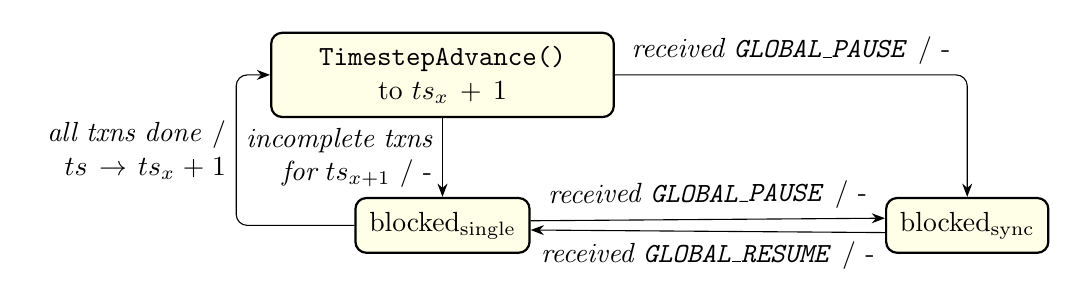
\begin{tikzpicture}[
		state/.style={draw, rectangle, rounded corners, fill=yellow!10, inner sep=5pt},
		every node/.style={thick},
	]

	% -- all states --

	\node [state,text width=4cm,align=center] (r) at (0, 0) {
		\texttt{TimestepAdvance()} \\ to $ts_{x} + 1$
	};
	\node [state,below=of r] (baop)
    {blocked\textsubscript{single}};
	% \node [state,below=of baop] (baoc)
	% {blocked\textsubscript{single}, committing};

	% \node [state] (bsync) at (12, -1.3) {blocked\textsubscript{sync}};
	\node [state,right=4.5cm of baop] (bsync) {blocked\textsubscript{sync}};
	% \node [state] (bsyncprep) at (baoc -| bsync) {blocked\textsubscript{single}, limited\_prepare};

	% -- regular 2PC edges --

	\draw (r) edge[-Stealth]
	node[left,text width=2.4cm,align=right]{
			\emph{incomplete txns \\for $ts_{x+1}$} / -
		} (baop);
	% \draw (baop) edge[-Stealth]
	% node[left,text width=2.7cm,align=right]{
	% 		\emph{uncommitted txns \\for $ts_{x+1}$} / -
	% 	} (baoc);

	% temporary, to visualize controls
	\coordinate (c1) at (-4.0, 0.5);
	\coordinate (c2) at (-4.0, -3.5);

	% \draw[-Stealth] (baoc.west) .. controls (c2) and (c1) .. node[above,sloped,rotate=180]{
	% 		% ABC
	% 		- / $ts \rightarrow ts_{x+1}$
	% 	} (r.west);

	% \filldraw[red] (c1) circle (2pt);
	% \filldraw[blue] (c2) circle (2pt);

	% -- blocked-sync edges --
	% \draw (bsync) edge[->] node[right,text width=6cm,align=center]{
	% 		\emph{received \texttt{GLOBAL\_RESUME}} / \\
	% 		allow prepares if txnseq \textless txnseq\textsubscript{resume}
	% 	} (bsyncprep);
	%
	\draw (bsync.185) edge[-Stealth] node[below]{
			\emph{received \texttt{GLOBAL\_RESUME}} / -
		} (baop.-3);

	% \draw[->,bend angle=10] (bsyncprep) edge[->,bend left]
	% node[below,sloped,text width=3cm,align=center]{
	% 		\emph{uncommitted txns for $ts_{x+1}$} / -
	% 	} (baoc.south);
	%
	% -- global pause edges --
	% \draw[-Stealth,bend angle=15] (r.east) to[bend left] node[above,sloped]{
	% 	\emph{received \texttt{GLOBAL\_PAUSE}} / -
	% } (bsync);

	\draw[-Stealth, rounded corners] (r) -| node[near start,above]{
		\emph{received \texttt{GLOBAL\_PAUSE}} / -
		} (bsync);

	\draw (baop.3) edge[-Stealth] node[above,sloped]{
			\emph{received \texttt{GLOBAL\_PAUSE}} / -
		} (bsync.175);

	% \draw[-Stealth,bend angle=15] (baoc) to[bend right] node[below,sloped]{
	% 	\emph{received \texttt{GLOBAL\_PAUSE}} / -
	% } (bsync.205);

	% \draw[-Stealth, rounded corners] (baoc) -| node[near start,below]{
	% 		\emph{received \texttt{GLOBAL\_PAUSE}} / -
	% 	} (bsync);

	%
	% \draw[->,bend angle=13,postaction={decorate,decoration={
	% 					raise=1ex,text along path, text align=center,text={
	%              |\itshape|received GLOBAL\_PAUSE
	%          }}}] (baoc) to[bend right] (bsync);
  % \draw[-Stealth, rounded corners] (baoc.west) |- ++(-2cm,0) |- (r) ;
  \draw[-Stealth, rounded corners] 
    (baop.west) -- ++(-1.5cm,0) |- (r.west) 
    node[near start,left,text width=2.4cm,align=right] {
      \emph{all txns done} / $ts \rightarrow ts_x + 1$
  };
\end{tikzpicture}
\end{document}
